\documentclass[
  jou,
  floatsintext,
  longtable,
  nolmodern,
  notxfonts,
  notimes,
  colorlinks=true,linkcolor=blue,citecolor=blue,urlcolor=blue]{apa7}

\usepackage{amsmath}
\usepackage{amssymb}




\RequirePackage{longtable}
\RequirePackage{threeparttablex}

\makeatletter
\renewcommand{\paragraph}{\@startsection{paragraph}{4}{\parindent}%
	{0\baselineskip \@plus 0.2ex \@minus 0.2ex}%
	{-.5em}%
	{\normalfont\normalsize\bfseries\typesectitle}}

\renewcommand{\subparagraph}[1]{\@startsection{subparagraph}{5}{0.5em}%
	{0\baselineskip \@plus 0.2ex \@minus 0.2ex}%
	{-\z@\relax}%
	{\normalfont\normalsize\bfseries\itshape\hspace{\parindent}{#1}\textit{\addperi}}{\relax}}
\makeatother




\usepackage{longtable, booktabs, multirow, multicol, colortbl, hhline, caption, array, float, xpatch}
\usepackage{subcaption}
\renewcommand\thesubfigure{\Alph{subfigure}}
\setcounter{topnumber}{2}
\setcounter{bottomnumber}{2}
\setcounter{totalnumber}{4}
\renewcommand{\topfraction}{0.85}
\renewcommand{\bottomfraction}{0.85}
\renewcommand{\textfraction}{0.15}
\renewcommand{\floatpagefraction}{0.7}

\usepackage{tcolorbox}
\tcbuselibrary{listings,theorems, breakable, skins}
\usepackage{fontawesome5}

\definecolor{quarto-callout-color}{HTML}{909090}
\definecolor{quarto-callout-note-color}{HTML}{0758E5}
\definecolor{quarto-callout-important-color}{HTML}{CC1914}
\definecolor{quarto-callout-warning-color}{HTML}{EB9113}
\definecolor{quarto-callout-tip-color}{HTML}{00A047}
\definecolor{quarto-callout-caution-color}{HTML}{FC5300}
\definecolor{quarto-callout-color-frame}{HTML}{ACACAC}
\definecolor{quarto-callout-note-color-frame}{HTML}{4582EC}
\definecolor{quarto-callout-important-color-frame}{HTML}{D9534F}
\definecolor{quarto-callout-warning-color-frame}{HTML}{F0AD4E}
\definecolor{quarto-callout-tip-color-frame}{HTML}{02B875}
\definecolor{quarto-callout-caution-color-frame}{HTML}{FD7E14}

%\newlength\Oldarrayrulewidth
%\newlength\Oldtabcolsep


\usepackage{hyperref}




\providecommand{\tightlist}{%
  \setlength{\itemsep}{0pt}\setlength{\parskip}{0pt}}
\usepackage{longtable,booktabs,array}
\usepackage{calc} % for calculating minipage widths
% Correct order of tables after \paragraph or \subparagraph
\usepackage{etoolbox}
\makeatletter
\patchcmd\longtable{\par}{\if@noskipsec\mbox{}\fi\par}{}{}
\makeatother
% Allow footnotes in longtable head/foot
\IfFileExists{footnotehyper.sty}{\usepackage{footnotehyper}}{\usepackage{footnote}}
\makesavenoteenv{longtable}

\usepackage{graphicx}
\makeatletter
\newsavebox\pandoc@box
\newcommand*\pandocbounded[1]{% scales image to fit in text height/width
  \sbox\pandoc@box{#1}%
  \Gscale@div\@tempa{\textheight}{\dimexpr\ht\pandoc@box+\dp\pandoc@box\relax}%
  \Gscale@div\@tempb{\linewidth}{\wd\pandoc@box}%
  \ifdim\@tempb\p@<\@tempa\p@\let\@tempa\@tempb\fi% select the smaller of both
  \ifdim\@tempa\p@<\p@\scalebox{\@tempa}{\usebox\pandoc@box}%
  \else\usebox{\pandoc@box}%
  \fi%
}
% Set default figure placement to htbp
\def\fps@figure{htbp}
\makeatother


% definitions for citeproc citations
\NewDocumentCommand\citeproctext{}{}
\NewDocumentCommand\citeproc{mm}{%
  \begingroup\def\citeproctext{#2}\cite{#1}\endgroup}
\makeatletter
 % allow citations to break across lines
 \let\@cite@ofmt\@firstofone
 % avoid brackets around text for \cite:
 \def\@biblabel#1{}
 \def\@cite#1#2{{#1\if@tempswa , #2\fi}}
\makeatother
\newlength{\cslhangindent}
\setlength{\cslhangindent}{1.5em}
\newlength{\csllabelwidth}
\setlength{\csllabelwidth}{3em}
\newenvironment{CSLReferences}[2] % #1 hanging-indent, #2 entry-spacing
 {\begin{list}{}{%
  \setlength{\itemindent}{0pt}
  \setlength{\leftmargin}{0pt}
  \setlength{\parsep}{0pt}
  % turn on hanging indent if param 1 is 1
  \ifodd #1
   \setlength{\leftmargin}{\cslhangindent}
   \setlength{\itemindent}{-1\cslhangindent}
  \fi
  % set entry spacing
  \setlength{\itemsep}{#2\baselineskip}}}
 {\end{list}}
\usepackage{calc}
\newcommand{\CSLBlock}[1]{\hfill\break\parbox[t]{\linewidth}{\strut\ignorespaces#1\strut}}
\newcommand{\CSLLeftMargin}[1]{\parbox[t]{\csllabelwidth}{\strut#1\strut}}
\newcommand{\CSLRightInline}[1]{\parbox[t]{\linewidth - \csllabelwidth}{\strut#1\strut}}
\newcommand{\CSLIndent}[1]{\hspace{\cslhangindent}#1}





\usepackage{newtx}

\defaultfontfeatures{Scale=MatchLowercase}
\defaultfontfeatures[\rmfamily]{Ligatures=TeX,Scale=1}





\title{\textbf{Introducing the Choice-Confidence (CHOCO) Model for
Bimodal Scales Data: Application to the Relationship between Reality
Beliefs about AI-Generated Faces and Beauty}}


\shorttitle{Choice-Confidence (CHOCO) Model}


\usepackage{etoolbox}









\authorsnames[{1,2},{1},{1}]{Dominique Makowski,Ana Neves,Andy Field}







\authorsaffiliations{
{School of Psychology, University of Sussex},{Sussex Centre for
Consciousness Science, University of Sussex}}




\leftheader{Makowski, Neves and Field}



\abstract{TO DO. }

\keywords{subjective scales, choice confidence model, reality beliefs,
AI-generated faces, attractiveness}

\authornote{\par{\addORCIDlink{Dominique
Makowski}{0000-0001-5375-9967}}\par{\addORCIDlink{Ana
Neves}{0009-0006-0020-7599}}\par{\addORCIDlink{Andy Field}{true}} 
\par{ }
\par{     \begin{tcolorbox}[enhanced jigsaw, colframe=quarto-callout-note-color-frame, rightrule=.15mm, bottomrule=.15mm, colback=white, arc=.35mm, breakable, toprule=.15mm, leftrule=.75mm, opacityback=0, left=2mm]

This preprint is a non-peer-reviewed work from the
\href{https://realitybending.github.io/}{\textbf{Reality Bending Lab}}.
\begin{center}
\includegraphics[width=0.2\linewidth,height=\textheight,keepaspectratio]{manuscript_files/mediabag/ReBeL_LogoOnly_hu114.png}
\end{center}

\end{tcolorbox}  Author roles were classified using the Contributor Role
Taxonomy (CRediT; https://credit.niso.org/) as follows:  Dominique
Makowski:   Conceptualization, Data curation, Formal Analysis, Funding
acquisition, Investigation, Methodology, Project
administration, Resources, Software, Supervision, Validation, Visualization, Writing
-- original draft; Ana Neves:   Data curation, Writing -- original
draft, Writing -- review \& editing; Andy Field:   Writing -- original
draft, Writing -- review \& editing}
\par{Correspondence concerning this article should be addressed
to Dominique
Makowski, Email: \href{mailto:D.Makowski@sussex.ac.uk}{D.Makowski@sussex.ac.uk}}
}

\usepackage{pbalance} 
\usepackage{float}
\makeatletter
\let\oldtpt\ThreePartTable
\let\endoldtpt\endThreePartTable
\def\ThreePartTable{\@ifnextchar[\ThreePartTable@i \ThreePartTable@ii}
\def\ThreePartTable@i[#1]{\begin{figure}[!htbp]
\onecolumn
\begin{minipage}{0.5\textwidth}
\oldtpt[#1]
}
\def\ThreePartTable@ii{\begin{figure}[!htbp]
\onecolumn
\begin{minipage}{0.5\textwidth}
\oldtpt
}
\def\endThreePartTable{
\endoldtpt
\end{minipage}
\twocolumn
\end{figure}}
\makeatother


\makeatletter
\let\endoldlt\endlongtable		
\def\endlongtable{
\hline
\endoldlt}
\makeatother

\newenvironment{twocolumntable}% environment name
{% begin code
\begin{table*}[!htbp]%
\onecolumn%
}%
{%
\twocolumn%
\end{table*}%
}% end code

\urlstyle{same}



\makeatletter
\@ifpackageloaded{tcolorbox}{}{\usepackage[skins,breakable]{tcolorbox}}
\@ifpackageloaded{fontawesome5}{}{\usepackage{fontawesome5}}
\definecolor{quarto-callout-color}{HTML}{909090}
\definecolor{quarto-callout-note-color}{HTML}{0758E5}
\definecolor{quarto-callout-important-color}{HTML}{CC1914}
\definecolor{quarto-callout-warning-color}{HTML}{EB9113}
\definecolor{quarto-callout-tip-color}{HTML}{00A047}
\definecolor{quarto-callout-caution-color}{HTML}{FC5300}
\definecolor{quarto-callout-color-frame}{HTML}{acacac}
\definecolor{quarto-callout-note-color-frame}{HTML}{4582ec}
\definecolor{quarto-callout-important-color-frame}{HTML}{d9534f}
\definecolor{quarto-callout-warning-color-frame}{HTML}{f0ad4e}
\definecolor{quarto-callout-tip-color-frame}{HTML}{02b875}
\definecolor{quarto-callout-caution-color-frame}{HTML}{fd7e14}
\makeatother
\makeatletter
\@ifpackageloaded{caption}{}{\usepackage{caption}}
\AtBeginDocument{%
\ifdefined\contentsname
  \renewcommand*\contentsname{Table of contents}
\else
  \newcommand\contentsname{Table of contents}
\fi
\ifdefined\listfigurename
  \renewcommand*\listfigurename{List of Figures}
\else
  \newcommand\listfigurename{List of Figures}
\fi
\ifdefined\listtablename
  \renewcommand*\listtablename{List of Tables}
\else
  \newcommand\listtablename{List of Tables}
\fi
\ifdefined\figurename
  \renewcommand*\figurename{Figure}
\else
  \newcommand\figurename{Figure}
\fi
\ifdefined\tablename
  \renewcommand*\tablename{Table}
\else
  \newcommand\tablename{Table}
\fi
}
\@ifpackageloaded{float}{}{\usepackage{float}}
\floatstyle{ruled}
\@ifundefined{c@chapter}{\newfloat{codelisting}{h}{lop}}{\newfloat{codelisting}{h}{lop}[chapter]}
\floatname{codelisting}{Listing}
\newcommand*\listoflistings{\listof{codelisting}{List of Listings}}
\makeatother
\makeatletter
\makeatother
\makeatletter
\@ifpackageloaded{caption}{}{\usepackage{caption}}
\@ifpackageloaded{subcaption}{}{\usepackage{subcaption}}
\makeatother

% From https://tex.stackexchange.com/a/645996/211326
%%% apa7 doesn't want to add appendix section titles in the toc
%%% let's make it do it
\makeatletter
\xpatchcmd{\appendix}
  {\par}
  {\addcontentsline{toc}{section}{\@currentlabelname}\par}
  {}{}
\makeatother

%% Disable longtable counter
%% https://tex.stackexchange.com/a/248395/211326

\usepackage{etoolbox}

\makeatletter
\patchcmd{\LT@caption}
  {\bgroup}
  {\bgroup\global\LTpatch@captiontrue}
  {}{}
\patchcmd{\longtable}
  {\par}
  {\par\global\LTpatch@captionfalse}
  {}{}
\apptocmd{\endlongtable}
  {\ifLTpatch@caption\else\addtocounter{table}{-1}\fi}
  {}{}
\newif\ifLTpatch@caption
\makeatother

\begin{document}

\maketitle


\setcounter{secnumdepth}{-\maxdimen} % remove section numbering

\setlength\LTleft{0pt}


\section{Introduction}\label{introduction}

Despite significant advancements in psychological science following the
replication crisis (\citeproc{ref-open2015estimating}{Collaboration,
2015}), its progress is still hindered by its sub-optimal (or
inappropriate) usage of statistical tools
(\citeproc{ref-makowski2023we}{Makowski \& Waggoner, 2023}). A prevalent
issue is the continued reliance on linear models that assume normally
distributed (Gaussian) data\footnote{More specifically, that the outcome
  is distributed according to a Normal distribution which parameters are
  expressed as a linear function of the predictors.} - as this
assumption often does not hold true for many types of psychological
outcomes. For instance, reaction times typically exhibit skewed
distributions, choices can be represented as binary variables, and count
data consists of strictly positive integers. Applying models that
presume normality and model the ``mean'' of the outcome variable can
lead to misinterpretation and potentially misleading conclusions when
applied indiscriminately. It is thus important that psychologists use
models that can best describe (or generate) the data they collect, to
fully exploit them and bring more nuance and accuracy to their
conclusions.

Among the most commonly collected data in psychology are responses on
subjective scales, such as Likert-type items or visual analog scales,
which exhibit some fundamental properties: these responses are bounded
(and can be rescaled to a 0-1 range) and frequently display clustering
at the extremes. Traditional linear models being ill-suited for such
data, researchers have turned to using Beta distributions to model this
data (instead of Gaussian), suited for continuous data within the (0,1)
interval (i.e., excluding extreme responses). To address the frequent
occurrence of exact zeros and ones (i.e., extreme values), zero-one
inflated beta (ZOIB) models have been developed
(\citeproc{ref-ospina2012general}{Ospina \& Ferrari, 2012}) to
accommodate the excess of boundary values by incorporating additional
components that model the probabilities of responses at 0 and 1 as a
separate, independent process.

\subsection{The Beta-Gate Model}\label{the-beta-gate-model}

The Beta-Gate model is a reparametrized Ordered Beta model
(\citeproc{ref-kubinec2023ordered}{Kubinec, 2023})\footnote{In the
  Ordered Beta model, the cutpoints on the log-scale are directly used
  as parameters, instead of being derived from \emph{pex} and
  \emph{bex}.} available in the \emph{cogmod} package in R
(https://github.com/DominiqueMakowski/cogmod), in which participants'
answers on bounded scales are conceptualized as latent responses that
can fall past a pair of probabilistic ``gates'' (or cutpoints) that
control whether the response is recorded as an extreme (0 or 1) or as a
nuanced, continuous value in between (Figure~\ref{fig-one}). These
distance of these gates from the edges of the scale varies based on two
interpretable parameters: \emph{pex} (the propensity by which people are
likely to answer extreme values), and \emph{bex}, a bias toward the
upper extreme (1) versus the lower (0). A person's internal response
that lies close to the edge might be ``caught'' by a gate and recorded
as an extreme, while others pass through to express a continuous
response (Beta-distributed with \(\mu\) (\emph{mu}) and \(\phi\)
(\emph{phi}) as its mean and precision parameters). The Beta-Gate model
is based on the idea that extreme values can emerge not just from a
fundamentally different underlying processes - as assumed in ZOIB models
- but from a common process governed by thresholds of decisiveness and
confidence.

\begin{figure}

\caption{\label{fig-one}The Beta-Gate Distribution is a reparametrized
ordered Beta model (Kubinec, 2023) that is governed by 4 parameters.
`Mu' and `phi' correspond to the mean and precision of the continuous
part of the distribution (between 0 and 1), and `pex' (propensity of
extremes) and `bex' (balance of extremes) indirectly control the
proportion of zeros and ones by specifying the location of the
``gates'', past which the latent response process is likely to generate
extreme values. Specifically, `pex' defines the total distance of both
gates from the extremes (in yellow), and `bex' determines the proportion
of the right gate distance relative to the left. In this example, the
total distance from the extremes is `pex' = 0.1, with 40\% (`bex' = 0.4)
of that distance being on the right (and 60\% on the left). The left
gate is thus located at 0.6, and the right at 1-0.04 = 0.96.}

\centering{

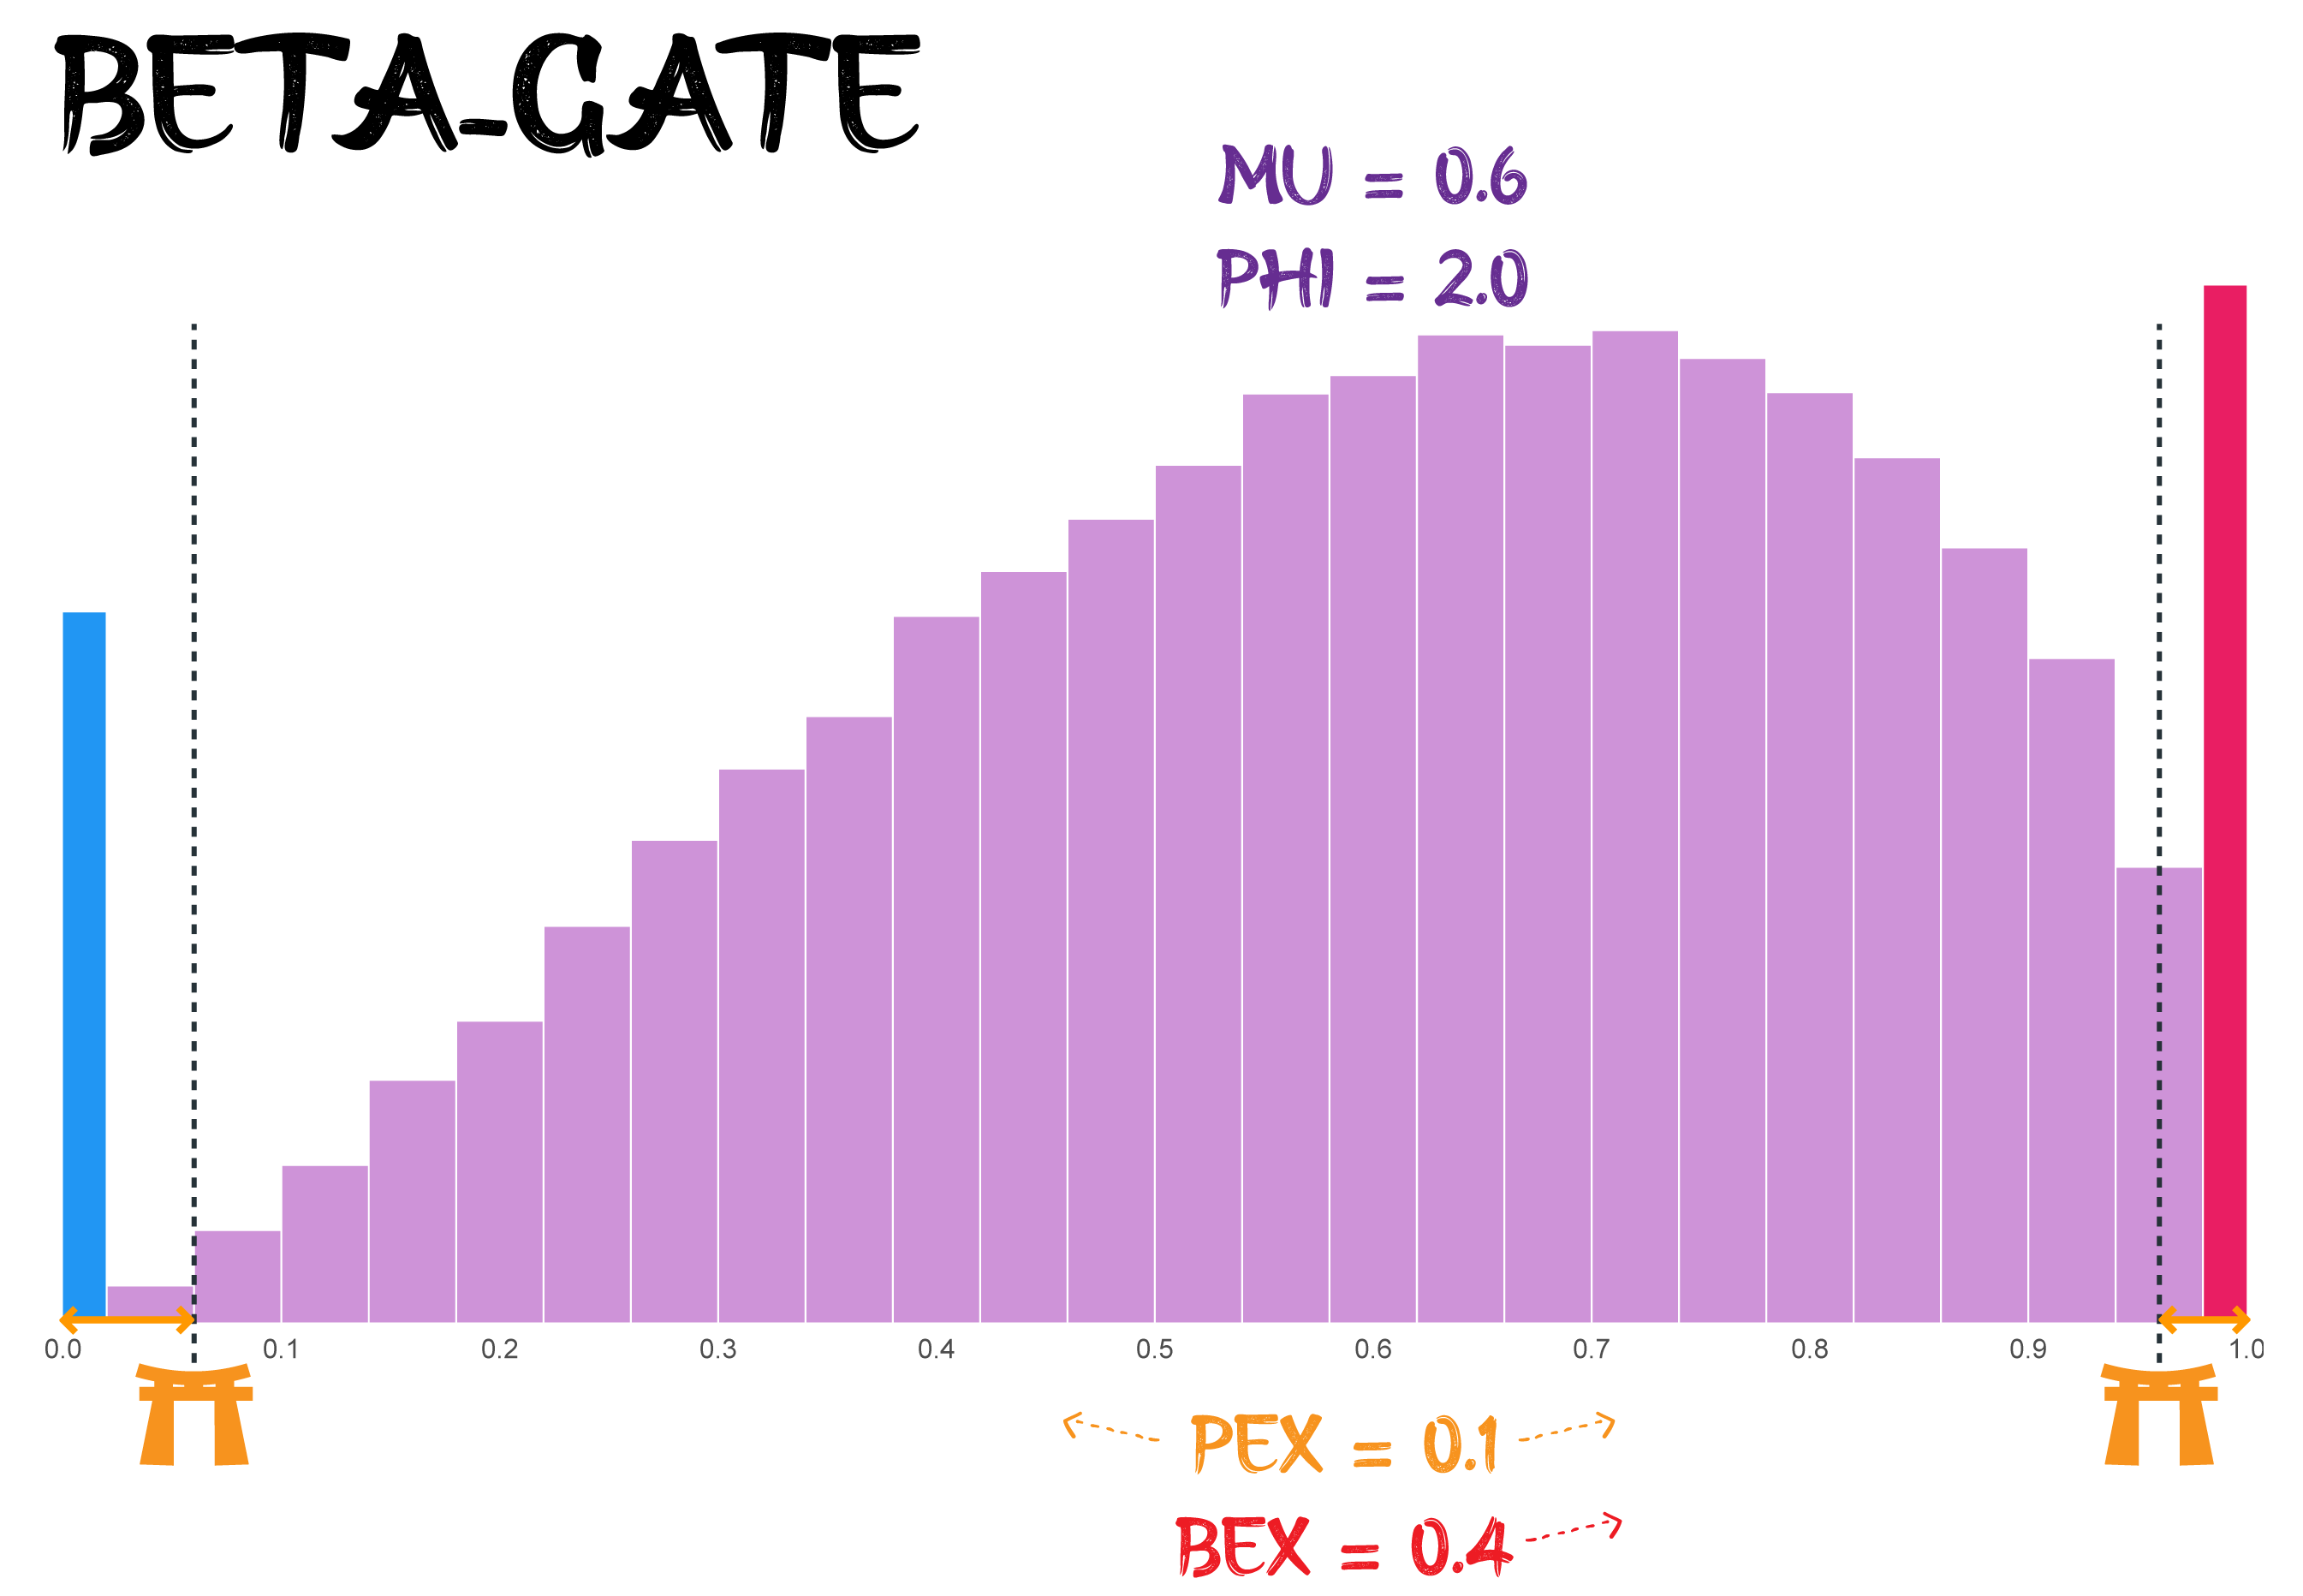
\includegraphics[width=1\linewidth,height=\textheight,keepaspectratio]{./figures/fig1.png}

}

\end{figure}%

Mathematically, the Beta-Gate distribution defines the observed outcome
\(x \in [0, 1]\) as a mixture of three components; a point mass at 0, a
point mass at 1, and a continuous Beta density over \(x \in (0,1)\),
scaled by the remaining probability mass. The probability of these
components are:

\begin{itemize}
\tightlist
\item
  \(P(x = 0) = \text{logistic}\left( \text{logit}(pex \cdot (1 - bex)) - \text{logit}(\mu) \right)\)
\item
  \(P(x = 1) = 1 - \text{logistic}\left( \text{logit}(1 - pex \cdot bex) - \text{logit}(\mu) \right)\)
\item
  \(P(x \in (0,1)) = 1 - P(x = 0) - P(x = 1)\)
\end{itemize}

The continuous part follows a Beta distribution with
parameters\footnote{Note that \emph{phi} is scaled in Beta-Gate models
  relative to the traditional mu/phi Beta particularization so that a
  phi of 1 corresponds to a uniform distribution - to facilitate setting
  priors on this parameter}:

\[
Beta(\alpha = \mu \cdot 2 \phi, \quad \beta = (1 - \mu) \cdot 2 \phi)
\]

\subsection{The Choice-Confidence (CHOCO)
Model}\label{the-choice-confidence-choco-model}

Decision-making is often conceptualized as involving distinct processes:
the choice itself, and the confidence associated with that choice. In
experimental paradigms, these can be somewhat disentangled by prompting
participants to make a discrete choice selection (e.g., ``True''
vs.~``False''), followed by a separate confidence rating. However, this
artificial separation makes its joint analysis difficulty, and may not
reflect real-world decision-making, where individuals often express both
choice and confidence simultaneously using a single, continuous scale.
In such scales, each side can represent a distinct latent category, and
the distance from the midpoint can indicates the level of confidence or
certainty. This integrated response format typically results in bimodal
distributions, with peaks corresponding to the mean confidence on either
side. Traditional beta regression models, which assume unimodal
distributions within the (0,1) interval, are ill-suited for such data.
One alternative is to transform the data into two variables a
posteriori: binarizing the side to represent choice and calculating the
absolute distance from the midpoint to represent confidence. These can
then be modeled separately, for instance, using logistic regression for
choice and beta regression for confidence (see
\citeproc{ref-makowski2025too}{Makowski, Te, et al., 2025} for an
example). While this approach can provide additional insights into
underlying mechanisms compared to a unique model, it assumes
psychological and statistical independence between choice and
confidence, which may not hold true in practice.

\begin{figure}

\caption{\label{fig-two}The CHOCO Model uses a mixture of Beta-Gate
distributions to model separately the right and left sides of the scale
(e.g., a rating of whether a statement was `Truth' vs.~`Lie'), as well
as their relative proportion. In this example, the participants are more
likely overall (p = 60\%) to select the right side of the scale (`Lie')
than the left (`Truth'). They are also more confident in their choice
(confright = 0.6 vs.~confleft = 0.3). Extreme values (zeros and ones)
are governed by the same mechanism as for Beta-Gate models.}

\centering{

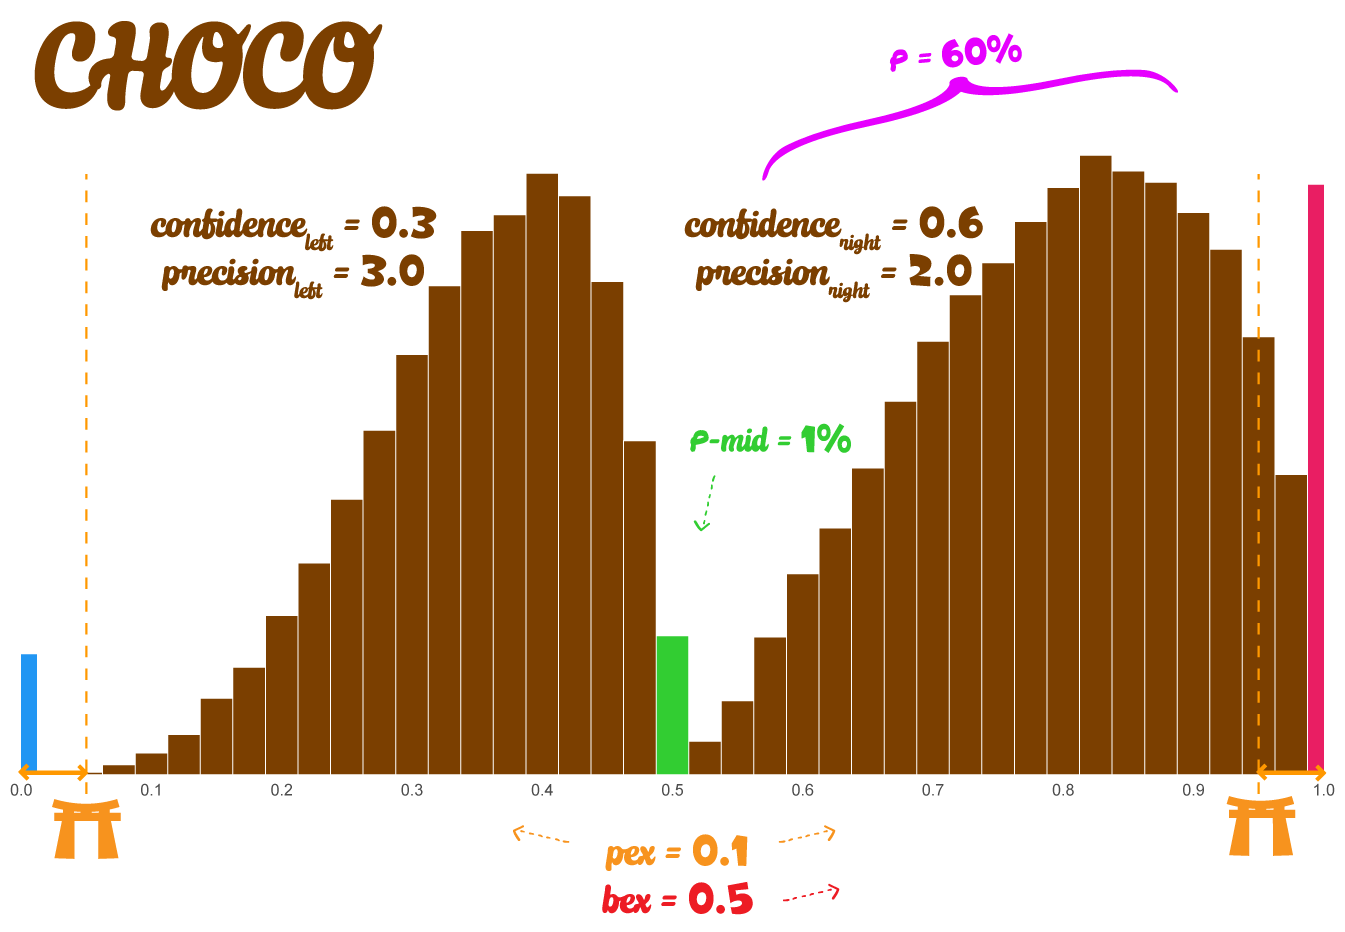
\includegraphics[width=1\linewidth,height=\textheight,keepaspectratio]{./figures/fig2.png}

}

\end{figure}%

To model data of subjective scales in which the left and right sides can
be conceptualized as two different choices (e.g., True/False,
Agree/Disagree, etc.) and the magnitude of the response (how much the
cursor is set away from the mid-point) as the confidence, we introduce
the Choice-Confidence (CHOCO) model (Figure~\ref{fig-two}). It consists
of a three‐part mixture on \(x \in [0, 1]\):

\begin{itemize}
\tightlist
\item
  An (optional) point-mass at the midpoint \emph{mid} (typically 0.5) of
  weight \(p_{\text{mid}}\) for undecided or neutral responses.\\
\item
  A left-choice component governed by a Beta-Gate density on the
  rescaled variable \(x/mid\) with mean \emph{1 - confleft}, precision
  \emph{precleft}, and boundary-excess parameter \emph{pex(1 - bex)}.\\
\item
  A right-choice component governed by a Beta-Gate density on the
  rescaled variable \((x - mid)/(1 - mid)\) with mean \emph{confright},
  precision \emph{precright}, and boundary-excess parameter \emph{pex x
  bex}.
\end{itemize}

The overall probability of the right choice (relative to the left
choice) is controlled by a main parameter \emph{p}. The full CHOCO
density is:

\[
\small
\begin{cases}
pmid, & x = mid, \\[6pt]
(1 - pmid)(1 - p)\,\dfrac{1}{mid} \cdot \mathrm{BetaGate}\left(\dfrac{x}{mid}\right), & 0 < x < mid, \\[6pt]
(1 - pmid)\,p\,\dfrac{1}{1 - mid} \cdot \mathrm{BetaGate}\left(\dfrac{x - mid}{1 - mid}\right), & mid < x < 1. \\
\end{cases}
\]

By coupling choice probability \(p\), midpoint mass \(p_{\text{mid}}\),
and side‐specific Beta-Gate parameters (\(conf\), \(prec\), \(pex\),
\(bex\)), CHOCO flexibly captures both bimodality and confidence
intensity in a single unified model. Despite this theoretical appeal, it
is unclear whether this heavily parametrized model can be estimated
reliably from data, and whether it can provide more useful insights than
simpler alternatives.

\subsection{Aim of the Present Study}\label{aim-of-the-present-study}

\textbf{Study 1} aims to evaluate the CHOCO model's ability to better
capture subjective scale responses that (potentially) reflect an
underlying discrete choice, in comparison to existing models such as the
ZOIB and Beta-Gate. Specifically, we will assess whether 1) CHOCO
provides improved model fit, 2) yields deeper insights into
population-level effects than traditional approaches (gender differences
in reality beliefs), and 3) allows for the reliable estimation of
interpretable individual-level parameters through random effects.
\textbf{Study 2} will apply this model to more subtle effects, such as
the effect perceived facial attractiveness on reality judgments, and
test the ability to fit alternative data structures (scales with ordinal
response options and mid-points). To this end, we analyze data from two
separate studies in which participants judged whether a face image was
AI-generated (``fake'') or a real photograph.

\section{Study 1}\label{study-1}

In today's post-truth era, the proliferation of advanced AI technologies
has made it increasingly challenging to distinguish between authentic
and synthetic media, bearing significant implications for information
integrity and public trust
(\citeproc{ref-lewandowsky2017beyond}{Lewandowsky et al., 2017}). As
traditional cues become less reliable (e.g., visual glitches and
artefacts in generated images; formulaic generated text, etc.), people
increasingly depend on contextual information and cognitive heuristics
to assess authenticity, a process referred to as ``simulation
monitoring'' (\citeproc{ref-makowski2019phenomenal}{Makowski, Sperduti,
et al., 2019}).

This reliance on alternative epistemological sources is particularly
pronounced under conditions of high ambiguity, where the
decontextualization of information, especially prevalent in online
environments, complicates authenticity assessments. An open question in
this domain is the extent to which reality judgments are influenced by
the stimuli themselves versus stable individual characteristics like
personality, expectations or expertise - or transient
psychophysiological states (\citeproc{ref-makowski2025too}{Makowski, Te,
et al., 2025}).

Images of faces - socially and perceptually rich stimuli for which
AI-generation has been particularly successful - are a paradigmatic
example that have been used to investigate reality judgments
(\citeproc{ref-azevedo2020body}{Azevedo et al., 2020};
\citeproc{ref-makowski2025too}{Makowski, Te, et al., 2025};
\citeproc{ref-nightingale2022ai}{Nightingale \& Farid, 2022};
\citeproc{ref-tucciarelli2022realness}{Tucciarelli et al., 2022}).
Studies asking participants to judge whether face images are real or
artificially generated reveal that such judgments can be shaped by
low-level features (e.g., clarity, symmetry), higher-level attributes
(e.g., attractiveness, trustworthiness), and interindividual
variability. In the present study, we apply the CHOCO model to such data
to evaluate its capacity to recover interpretable parameters related to
individual-level determinants of reality beliefs.

\subsection{Methods}\label{methods}

\subsubsection{Participants}\label{participants}

Using the open-accss data from Makowski, Te, et al.
(\citeproc{ref-makowski2025too}{2025}), we included all heterosexual and
bisexual (as these two groups did not seem to differ based on
preliminary analyses and were thus grouped to maximize power) male and
female participants, for a final sample of 141 participants (Mean age =
28.4, SD = 9.0, range: {[}19, 66{]}; Sex: 47.5\% females). For each
participant, we included only stimuli of the opposite gender (i.e., all
89 female faces for men and 20 male faces for women).

\subsubsection{Procedure}\label{procedure}

In the first phase, participants viewed 109 neutral-expression
photographs of faces (random order, display time of 3 s) from the
American Multiracial Face Database (AMFD,
\citeproc{ref-chen2021broadening}{Chen et al., 2021}). After each image,
participants rated the face on trustworthiness, familiarity,
attractiveness, and beauty using visual analog scales. In the second
phase, participants were informed that ``about half of the previously
seen images were AI-generated''. The same faces were presented again in
a new random order (same display time), followed by ratings of
``reality'' (whether they believed the image was fake - left anchor - or
real - right anchor).

\subsubsection{Data Analysis}\label{data-analysis}

We fitted 3 models to predict the reality ratings: a ZOIB model, a
Beta-Gate model, and the CHOCO model. For all models and each parameter,
the full formula was entered:
\(Real\sim Sex + (1 | Participant) + (1 | Item)\) (with Sex as the main
predictor and participants and items entered as random intercepts). The
models were run using \emph{brms}
(\citeproc{ref-burkner2017brms}{Bürkner, 2017}) R package, and analyzed
using the \emph{easystats} collection of packages
(\citeproc{ref-ludecke2020extracting}{Lüdecke et al., 2020};
\citeproc{ref-makowski2025modelbased}{Makowski, Ben-Shachar, et al.,
2025}; \citeproc{ref-patil2022datawizard}{Patil et al., 2022}). To
maximize the comparability across models We used the default priors
(uniform) for all models, and we ran 16 chains of 1400 iterations each
on the University of Sussex High-Performance Computing (HPC) cluster.

Model comparisons were performed using the \emph{loo} R package
(\citeproc{ref-vehtari2017practical}{Vehtari et al., 2017}), which
computes the Widely Applicable Information Criterion (WAIC) and
estimates the Expected Log Predictive Density (ELPD) and penalizes the
number of parameters. We assessed model performance by examining ELPD
differences and their standard errors (SE), reporting corresponding
\emph{p}-values to determine significant differences in predictive
accuracy.

For the population-level effects, we will consider significant and
report (using the median of the posterior distribution) effects for
which the 95\% Credible Interval (CI) does not include zero (and when
the probability of direction \emph{pd} is \textgreater{}
\textasciitilde97\%, \citeproc{ref-makowski2019indices}{Makowski,
Ben-Shachar, et al., 2019}). For the individual-level parameters (i.e.,
the random intercepts of each parameter for each participant and each
item), we will first analyze their reliability using the
Variance-Over-Uncertainty Ratio index (\emph{D-vour}). This index,
implemented in the \emph{performance} package
(\citeproc{ref-ludecke2021performance}{Lüdecke et al., 2021}), is
inspired by recent work on mixed models reliability
(\citeproc{ref-rouder2024hierarchical}{Rouder \& Mehrvarz, 2024};
\citeproc{ref-williams2021beneath}{Williams et al., 2021}), and
corresponds to the normalized ratio of observed variability to
uncertainty in random effect estimates, defined as:

\[
D_{\text{vour}} = \frac{\sigma_B^2}{\sigma_B^2 + \mu_{\text{SE}}^2}
\]

Where \(\sigma_B^2\) is the between-group variability (computed as the
SD of the random effect point-estimates) and \(\mu_{\text{SE}}^2\) is
the mean squared uncertainty in random effect estimates (i.e., the
average uncertainty). We use as \emph{D-vour} = 0.666 as the threshold
for moderately reliable random effect estimates, which corresponds to a
2:1 ratio of between-group variance to uncertainty.

Finally, we will run a correlation analysis of the models'
individual-level estimates against ``empirical'' (indices computed
directly on the observed data), including the empirical \emph{p}, the
overall \emph{conf}, \emph{pex} and \emph{bex} (respectively calculated
as \(P(y > 0.5)\); \(mean(|y - 0.5|)\); \(P(y \in [0, 1])\); and
\(P(y == 1) / P(y \in [0, 1])\)), assessing whether the model's estimate
are in-line with easily interpretable indices.

\subsection{Results}\label{results}

The reproducible code and full result report are available at
https://github.com/RealityBending/FictionChoco.

\subsubsection{Model Comparison}\label{model-comparison}

\begin{figure*}[!htbp]

{\caption{{Top: Model comparison revealed that the CHOCO model was a
significantly better fit for the data (raw distribution in purple)
compared to a ZOIB or Beta-Gate models, capturing its bimodal
distribution. Bottom: the CHOCO model can be set to estimate effect on
any of its parameters, such as the overall probability of responding on
one side as well as the confidence in both choices. We illustrate this
by showing the effect of Sex on the distribution of reality beliefs
based on a CHOCO model.}{\label{fig-three}}}}

\includegraphics[width=1\linewidth,height=\textheight,keepaspectratio]{./figures/fig3.png}

\end{figure*}

The models did converge without divergent transitions, and the effective
sample size was sufficient for all parameters (all
\(n_{\text{eff}} > 1000\)). The difference in predictive accuracy, as
indexed by Expected Log Predictive Density (ELPD-WAIC), suggests that
the \emph{CHOCO} is the best model (\(ELPD = -203.54\)), followed by
\emph{Beta-Gate} (\(\Delta_{ELPD} = -1794.57 \pm 63.12, ~p < .001)\) and
\emph{ZOIB} (\(\Delta_{ELPD} = -1833.59 \pm 63.52, ~p < .001\)). See
Figure~\ref{fig-three} for the posterior predictive checks, showing that
only the CHOCO model managed to capture the bimodal distribution of
data.

\subsubsection{Effect of Sex}\label{effect-of-sex}

The ZOIB model suggested that women had higher mean scores of reality
beliefs
(\(\mu_{~\text{Female}} = 0.20,~95\%~ CI~[0.03, 0.37], ~pd = 98.77\%\)),
less extreme values
(\(zoi_{~\text{Female}} = -1.24,~95\%~ CI~[-2.46, -0.07], ~pd = 98.25\%\))
but more ones relative to zeros
(\(coi_{~\text{Female}} = 1.63,~95\%~ CI~[0.70, 2.56], ~pd = 99.97\%\)).

The Beta-Gate model similarly suggested that women had higher mean
scores of reality beliefs
(\(\mu_{~\text{Female}} = 0.21,~95\%~ CI~[0.02, 0.40], ~pd = 98.52\%\)),
less extreme values
(\(pex_{~\text{Female}} = -1.34,~95\%~ CI~[-2.56, -0.17], ~pd = 98.75\%\)),
and a greater tendency to answer one relative to zero
(\(bex_{~\text{Female}} = 1.13,~95\%~ CI~[0.34, 1.91], ~pd = 99.76\%\)).

The CHOCO model shows that women had a higher probability \emph{p} of
judging faces as real
(\(P_{~\text{Female}} = 0.45,~95\%~ CI~[0.05, 0.86], ~pd = 98.54\%\)),
but are not more confident when doing so
(\(confright_{~\text{Female}} = -0.13,~95\%~ CI~[-0.47, 0.21], ~pd = 77.73\%\)).
However, they were less confident when answering that an image was
AI-generated
(\(confleft_{~\text{Female}} = -0.53,~95\%~ CI~[-0.89, -0.17], ~pd = 99.84\%\)).
There were also less likely to produce extreme answers
(\(pex_{~\text{Female}} = -1.19,~95\%~ CI~[-2.40, 0.01], ~pd = 97.64\%\)),
but no strong evidence supporting a directional bias was observed
(\(bex_{~\text{Female}} = 0.48,~95\%~ CI~[-0.12, 1.09], ~pd = 94.32\%\)).

Across all these models, no effect of Sex on the precision parameter was
observed.

\subsubsection{Individual-Level
Parameters}\label{individual-level-parameters}

\begin{figure*}[!htbp]

{\caption{{Top: the participant and item-level estimates for the CHOCO
parameters, under the distribution of their point-estimates. Reliable
effects are characterised by a higher between-group variability relative
(the dispersion of the distribution of point-estimates) to its
within-group variability (the average uncertainty of individual
estimates represented by the error bar). For example, inter-individual
variability in the parameters reflecting the confidence in left and
right choices is reliably capture, as opposed to the inter-individual
variability in the `bex' parameter. Bottom: correlation matrix between
participant-level estimates from different models and empirical indices
(e.g., the raw proportion of responses on the right per participant).
The CHOCO parameters are easily interpretable, strongly correlating with
their empirical counterparts.}{\label{fig-four}}}}

\includegraphics[width=0.95\linewidth,height=\textheight,keepaspectratio]{./figures/fig4.png}

\end{figure*}

The ZOIB model estimated reliable variability in the participant's
\emph{phi} parameter (D-vour = 0.88) and \emph{zoi} parameter (D-vour =
0.85), as well as in the \emph{mu} parameter related to individual items
(D-vour = 0.82). Moderate reliability was also observed for items in the
\emph{coi} parameter (D-vour = 0.71) and for participants in the
\emph{mu} parameter (D-vour = 0.69). The Beta-Gate model yielded similar
results: a high reliability of participant's \emph{phi} parameter
(D-vour = 0.88), \emph{pex} parameter (D-vour = 0.85). The \emph{mu}
parameter's variability was reliably captured for items (D-vour = 0.85)
and moderately for participants (D-vour = 0.72).

The CHOCO model yielded reliable estimates (Figure~\ref{fig-four}) for
all parameters except \emph{bex} for participants (\emph{confright}
D-vour = 0.94, \emph{confleft} D-vour = 0.91, \emph{pex} D-vour = 0.79,
\emph{p} D-vour = 0.73, \emph{precright} D-vour = 0.77, \emph{precleft}
D-vour = 0.67). Item's variability was primarily reflected through the
\emph{p} parameter (D-vour = 0.86).

Finally, the empirical average correlated the most strongly with CHOCO's
\emph{p} (r = .86), rather than ZOIB's \emph{mu} (r = .77) or
Beta-Gate's \emph{mu} (r = .82). The empirical overall confidence was
the strongest correlated with CHOCO's \emph{confright} (r = .91),
followed by ZOIB's \emph{phi} (r = -.86), Beta-Gate's phi (r = -.83),
and other CHOCO's parameters. The empirical proportion of ``right''
answer \emph{p} correlated the strongest with CHOCO's \emph{p} (r =
0.94), followed by Beta-Gate's \emph{mu} (r = .82) and ZOIB's \emph{mu}
(r = .77). The empirical \emph{pex} correlated the strongest with ZOIB's
\emph{zoi} (r = .90), and Beta-Gate's \emph{pex} (r = .90), and CHOCO's
\emph{pex} (r = .88). Of note that the parameters of Beta-Gate and ZOIB
correlate almost perfectly, underlining their empirical similarity
despite a different parametrization.

\subsection{Discussion}\label{discussion}

Study 1 revealed that the Choice-Confidence (CHOCO) model was a much
better fit for bimodal bounded data, compared to other alternatives like
the Zero-and-One Inflated Beta (ZOIB) and Beta-Gate (Ordered Beta)
models. It also allowed for a deeper understanding through its
interpretable parameters, offering insights into possibly distinct
cognitive mechanisms, such as the probability of answering real
vs.~fake, and the associated confidence in these two choices. This was
illustrated by modelling the effect of sex on all the CHOCO parameters.

Note that the observed gender differences are primarily presented as a
proof-of-principle, to showcase the model's ability to capture
group-level effects and to provide deeper insights compared to other
models. However, given that they were based on different items (female
and male faces), these differences might just be a reflection of stimuli
characteristics rather than true sex dymorphism in the formation of
reality beliefs.

Finally, we also show that the CHOCO model was able to capture reliable
and interpretable individual-level parameters, supporting its value to
measure inter-individual differences. An interesting dissociation
emerged between participant- and item-level variability: the latter
seemed mostly to be represented in the \emph{p} parameter, while
participants reliably varied in most of the components (aside from
\emph{bex}). This could suggest that external item characteristics
primarily influence the probability of being judged as real vs.~fake,
while the expressed confidence is first and foremost an individual
characteristic.

\section{Study 2}\label{study-2}

The explosion of accessibility of state-of-the-art AI tools has made it
effortless to generate realistic images, including human faces that are
often indistinguishable from real ones
(\citeproc{ref-bozkir2024can}{Bozkir et al., 2024};
\citeproc{ref-miller2023ai}{Miller et al., 2023};
\citeproc{ref-nightingale2022ai}{Nightingale \& Farid, 2022}). These
synthetic visuals are flooding the cyberspace across various domains,
such as art, advertising and entertainment, to education and
information. This technological advancement carries an important
potential for misuse, such as in disinformation campaigns, scams (e.g.,
AI-bots, identity theft), and abuse. The democratization of such
technology raises pressing concerns about the value of authenticity and
the potential erosion of media trust in our increasingly
\emph{post-truth} society.

In this evolving landscape, understanding the cognitive mechanisms that
underpin our judgments of reality becomes paramount. Despite the
increasing prevalence of digitally altered or AI-generated content,
humans still rely on certain heuristics to assess authenticity. One such
heuristic might be facial attractiveness. Attractiveness appraisals are
known to be automatic and unconscious (\citeproc{ref-hou2023neural}{Hou
et al., 2023}; \citeproc{ref-hung2016unconscious}{Hung et al., 2016};
\citeproc{ref-luo2019robust}{Luo et al., 2019}), and carry strong
real-life consequences, as demonstrated by the large body of literature
on the ``beauty premium''\footnote{As an eloquent example, Monk Jr et
  al. (\citeproc{ref-monk2021beholding}{2021}) reported in a large
  representative US sample that the magnitude of earnings disparities
  among white women along the perceived attractiveness continuum exceeds
  in magnitude the canonical black-white race gap.}
(\citeproc{ref-gulati2024beautiful}{Gulati et al., 2024};
\citeproc{ref-kukkonen2024beauty}{Kukkonen et al., 2024};
\citeproc{ref-little2021facial}{Little, 2021};
\citeproc{ref-pandey2021face}{Pandey \& Zayas, 2021}).

Although its role as a potential modulator of reality beliefs remains
under-explored, Makowski, Te, et al.
(\citeproc{ref-makowski2025too}{2025}) found significant associations
between participants' realness ratings and facial attractiveness, with a
potential sexual dymorphism: male participants judged attractive faces
as being likely more real, whereas evidence suggested a milder and
quadratic (U-shaped) relationship between attractiveness and reality
beliefs for females. These findings offer a complementary perspective to
those of Miller et al. (\citeproc{ref-miller2023ai}{2023}), who reported
that participants used attractiveness as a distinguishing cue between
real and AI-generated faces. These results highlight a possible
bidirectional and context-dependent influence of attractiveness on
reality judgments, of which the exact shape needs further investigation.

\subsection{Methods}\label{methods-1}

\subsubsection{Participants}\label{participants-1}

The first sample includes the same participants as study 1 (N = 141, see
above). For the second sample (data and preprocessing information
available at https://github.com/RealityBending/FakeFace2), 248
participants were initially recruited through academic platforms (SONA
and SurveySwap). We removed 15 participants with data suggesting
low-effort responding as well as those (N=16) that did not believe in
the experimental manipulation and were fully confident that all images
were real or fake. Similarly to the first sample, we included all hetero
and bisexual participants and stimuli from the opposite gender,
resulting in a final sample included 189 participants (Mean age = 28.4,
SD = 14.0, range: {[}18, 69{]}; Sex: 76.2\% females). The study was
approved by the University of Sussex Ethics Board (ER/ST633/1).

\subsubsection{Procedure}\label{procedure-1}

For the second sample, the procedure was relatively similar to that of
the first sample (described above in Study 1) with a few key
differences.

The main difference was the introduction of an experimental
manipulation: while for sample 1, participants were simply informed of
the presence of AI-generated stimuli among photographs (not providing
information as to specifically which image), the reality beliefs were
directly manipulated in sample 2. At the beginning of the experiment, a
cover story presented the study as a partnership with an AI startup
aimed at testing the quality of a new face AI-generation algorithm.
Following that, participants would see the 109 neutral-expression
photographs from the AMFD database (1 s), each preceded by a randomly
assigned textual cue indicating whether the image was ``AI-generated''
or ``Photograph'' (2 s). Ratings of attractiveness, beauty and
trustworthiness were collected after each image.

This phase of the experiment concluded with multi-choice questions
asking participants to indicate whether they believed in the cover
story. The second phase would start with a new set of instructions
(falsely) revealing that the cues were ``mixed up'' (shuffled randomly),
and that they would now be presented with the faces again (1 s) followed
by an assessment of their own beliefs about whether the image was real
or fake.

The second main difference was the subjective ratings' format, collected
using a 7-point Likert scale ranging from 0 to 6 (which included a clear
midpoint option), rather than a visual analog scale for sample 1. The 3
buttons on the left side (0, 1, 2) were colored in red and corresponded
to the more-or-less pronounced belief that the image was
``AI-generated'', the 3 values on the right (4, 5, 6) for ``Photograph''
were colored in green, and the middle value (3), representing an
undecided option, was colored in yellow.

\subsubsection{Data Analysis}\label{data-analysis-1}

To compare the benefits of CHOCO models to a ``traditional'' analytic
approach, we started by fitting a frequentist linear mixed model to
predict reality beliefs with the formula
\(Real\sim Sex / poly(Attractive, 2) + (poly(Attractive, 2)|Participant) + (1|Item)\).
The second degree orthogonal polynomial term was included to allow for
potentially non-linear relationships (note that the first and second
degree effects of orthogonal polynomials can be interpreted
independently as the linear part and the ``curvy'' part of the
relationship). For the CHOCO model, mildly informative and
effect-agnostic (i.e., centered at zero) priors were used. The same
formula was used for all parameters, except that items were only
included as random effects for \emph{p}, and participants were not
included for \emph{bex} (based on the reliability analysis of Study 1).

For sample 2, the analysis was based on that of Sample 1. The main
differences are 1) the inclusion of the ``Condition'' (whether the
picture was presented as ``Real'' of ``Fake'' in the first phase of the
experiment) as an additional predictor (entered as the only random slope
for all participant random effects); 2) the inclusion of an additional
parameters, \emph{pmid}, modelling the probability of answering the
middle-point of the Likert scale (representing an ``undecided'' option);
3) as they were effectively only 3 distinct values on each side of the
scale, and to showcase the flexibility of the CHOCO model, we decided to
\emph{not} treat the extreme values as 0 and 1 (and model them via the
separate parameters \emph{pex} and \emph{bex}, which would distributions
to be estimated from only 2 values), but instead to treat them as part
of the continuous distribution. The 7 response options were rescaled to
be evenly spaced between 0 and 1 excluded (i.e., {[}0.125, 0.875{]}).
The \emph{pex} and \emph{bex} parameters were fixed to 0, making for a
slightly more parsimonious model.

\subsection{Results}\label{results-1}

As the complete model parameters tables are available at
https://github.com/RealityBending/FictionChoco, we will focus on
reporting noteworthy findings below.

\subsubsection{Sample 1}\label{sample-1}

\begin{figure*}[!htbp]

{\caption{{The effect of attractiveness on reality beliefs. Top: the
effect of different levels of attractiveness (shades of red) on the
CHOCO distribution of the reality ratings in both samples, showing
primarily that, for male participants, more attractive faces were judged
more likely as a photograph rather than an AI-generated image. For the
second sample, stimuli that were during the initial viewing presented as
`AI-generated' are represented via a dotted line. Bottom: The impact of
attractiveness (x-axis) on different CHOCO distribution parameters, for
male and female participants (the AI-generated condition is added as a
transparent line for sample 2). Given the presence of polynomial terms,
significant effects are denoted by a symbol representing the shape of
the relationship (/ or \textbackslash{} for linear, U or inverse-U for
quadratic links).}{\label{fig-five}}}}

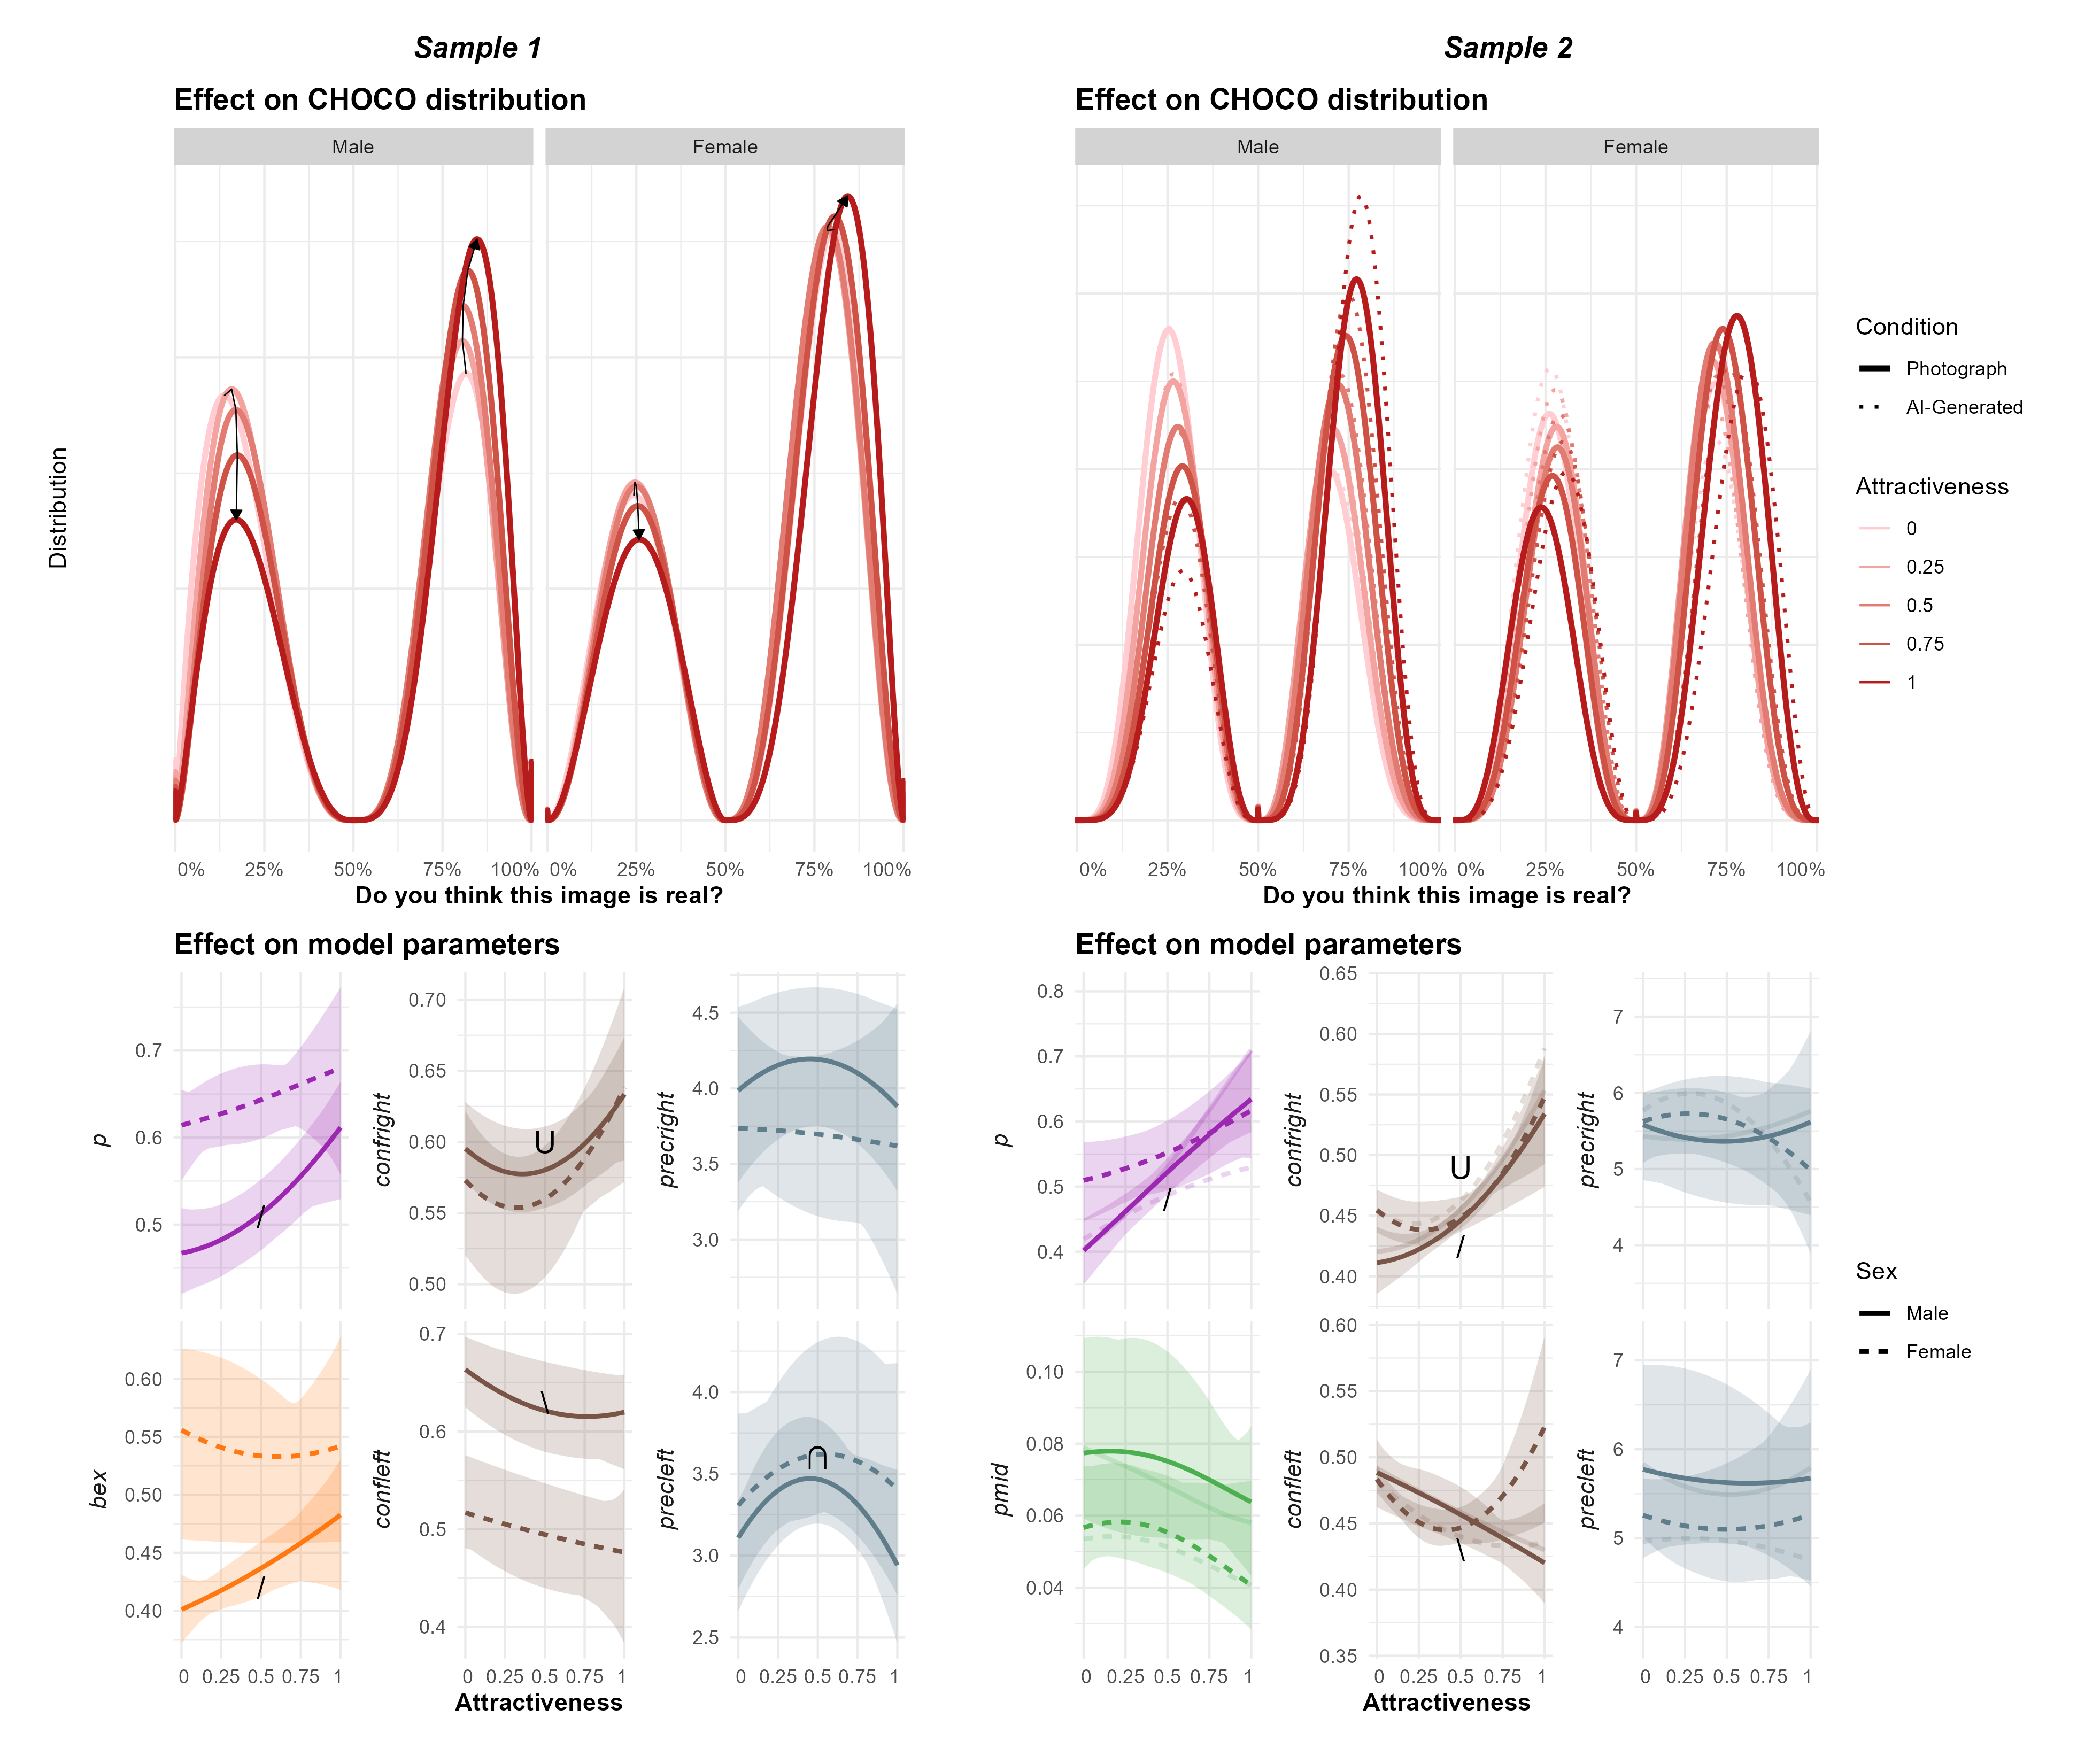
\includegraphics[width=1\linewidth,height=\textheight,keepaspectratio]{./figures/fig5.png}

\end{figure*}

In sample 1, the traditional approach suggested a significant linear
relationship between the mean level of ``Reality'' and attractiveness
for males only
(\(\beta_{~\text{poly1}}=3.42, ~95\%~CI [2.50, 4.34], ~p < .001\)), the
second largest effect being that of a quadratic link for women
(\(\beta_{~\text{poly2}}=1.82, ~95\%~CI [-0.27, 3.92], ~p = .09\)). The
CHOCO model revealed that, for males only, attractiveness had a
significantly positive linear relationship with the probability \emph{p}
of judging faces as real
(\(P_{~\text{poly1}}=13.64, ~95\%~CI [8.42, 18.99], ~pd = 100\%\)), but
a quadratic relationship with the confidence in real judgments
(\(confright_{~\text{poly2}}=3.70, ~95\%~CI [0.80, 6.40], ~pd = 99.53\%\)).
Attractiveness was also associated with less confidence in fake
judgments
(\(confleft_{~\text{poly1}}=-5.49, ~95\%~CI [-8.84, -2.11], ~pd =  99.92\%\)),
a quadratic relationship with left precision
(\(precleft_{~\text{poly2}}=-12.65    , ~95\%~CI [-24.59, -0.36], ~pd = 97.86\%\)),
and related linearly with a stronger bias towards extreme Real responses
(\(bex_{~\text{poly1}}=9.56    , ~95\%~CI [2.44, 16.73], ~pd = 99.55\%\)).
No significant relationship was found for females. The reliability of
the effect of attractiveness (the random slopes) was very low for all
parameters (D-vour \textless{} 0.01).

\subsubsection{Sample 2}\label{sample-2}

In Sample 2, the traditional approach suggested a significant linear
relationship between the mean level of ``Reality'' and attractiveness
for males
(\(\beta_{~\text{poly1}}=3.87, ~95\%~CI [2.91, 4.83], ~p < .001\)) and
females
(\(\beta_{~\text{poly1}}=1.88, ~95\%~CI [0.74, 3.01], ~p < .001\)), with
no effect of the Condition. The CHOCO model revealed that attractiveness
had a significantly positive linear relationship with the probability
\emph{p} of judging faces as real for males
(\(P_{~\text{poly1}}=18.44, ~95\%~CI [11.36, 25.31], ~pd = 100\%\)) and
females
(\(P_{~\text{poly1}}=9.08, ~95\%~CI [1.90, 16.35], ~pd = 99.27\%\)). It
also had a linear relationship with the confidence in real judgments for
males
(\(confright_{~\text{poly1}}=7.51, ~95\%~CI [3.90, 11.30], ~pd = 99.99\%\)),
as well as a significant quadratic relationship for females
(\(confright_{~\text{poly2}}=4.48, ~95\%~CI [0.74, 8.18], ~pd = 99.09\%\)).
Attractiveness also linearly decreased the confidence in fake judgments
only for males
(\(confleft_{~\text{poly1}}=-6.67, ~95\%~CI [-10.04, -3.38], ~pd = 100\%\)).
Marginal contrasts suggested that stimuli previously labelled as
photographs increased the probability \emph{p} of judging faces as real,
only for females
(\(P \Delta_{~\text{real - fake}}=0.06, ~95\%~CI [0.00, 0.11], ~pd = 98.36\%\)).

\subsubsection{Beauty}\label{beauty}

The same analysis was run for Beauty, which indicated the following
differences: \textbf{ANA: can you report the main differences?}

\subsection{Discussion}\label{discussion-1}

\textbf{WIP}

The fact that the effect was less obvious in women in the sample 1 might
be explained with power (less relevant items were included for women).

\section{General Discussion}\label{general-discussion}

\textbf{WIP}

This study introduces a new statistical model to analyze bimodal data,
which can be observed for instance when using subjective rating scales
in which the two sides correspond to a different ``choice'' (e.g.,
``false'' vs.~``true'', ``real'' vs ``fake''). The Choice-Confidence
(CHOCO) model conceptualizes the data as a mixture of two distributions,
one for each choice, and models the probability of choosing one or the
other as well as the degree of confidence in each choice. We validated
this model on real-life data by appling it to the reality beliefs of
Makowski, Te, et al. (\citeproc{ref-makowski2025too}{2025}), and showed
that it was able to capture the bimodal nature of the data and provides
a more accurate representation of the underlying processes than other
alternative approaches, including Zero-or-One inflated Beta (ZOIB)
models.

Little difference between Beauty and Attractiveness, aside that Beauty
revealed more effects in women. Why?

We demonstrated the flexibility of the CHOCO model, being usable in
analog scales as well as discrete ratings with a mid-point.

Likert-scales (with a limited number of discrete options) are commonly
used in psychology, and often modeled as continuous. While this fact has
spurred its own polarized debate (REFS), our position is that the model
used should ideally reflect the data \emph{generating} mechanism rather
than necessarily focus on the \emph{observed} data\footnote{Ideally, the
  data recording method should be aligned with the assumed generating
  mechanism, which is an experiment design issue rather than a
  statistical one.} - although the former cannot always be easily
inferred or known. For the data of Sample 2, we held the assumption that
the underlying latent distribution was CHOCO distributed (as there is no
reason to assume it would be different from Sample 1), treated as
continuous CHOCO-distributed data, despite the fact that it was
collected on a 7-point Likert scale. The motivation was to see if the
model could extrapolate and reliably estimate all the parameters based
on a limited number of data points but means in our case that,
effectively, each Beta distribution was extrapolated from the frequency
of only two unique values (or 3 for the no-extreme version). While this
is far from ideal, the CHOCO model still provided a better fit to the
data than alternative approaches. \textbf{TODO} However, it might have
lead to a lesser ability to detect finer grain changes, including
U-shaped relationships. Having 7-points (or 6 with no mid-value) is the
strict minimum to use the CHOCO model.

While our study was pertaining to \emph{simulation monitoring}, the
process of assessing and forming beliefs about the nature of external
stimuli (REF makowski phenomenological), we believe that it is part of
the mechanisms at play in the fabric of our sense of reality (REF
makowski thesis), alongside others, such as presence (the embodied
feeling of being physically ``in'' an experience) or \emph{reality
monitoring} (the process of distinguishing between internally generated
and externally perceived events, i.e., imagination vs.~perception).
Interestingly, recent studies about the latter support a possible
distinction at a neural level between \ldots{} and (binary) decision
making. (https://www.cell.com/neuron/fulltext/S0896-6273(25)00362-9).

Future studies should assess psychometric property liek the minimum
amount of data required to estimate and recover all parameters reliably.

Future studies should assess the ability of CHOCO models to also fit
unimodal distributions (so it can be used more generally), as well as
the benefits of more parsimonious parametrization (for instance, a
unique precision parameter controlling both the left and right sides, or
a linked confidence parameter e.g.~where \emph{confleft} is expressed as
a function of \emph{confright}).

\section{Data Availability}\label{data-availability}

Data, code and everything is available at
https://github.com/RealityBending/FictionChoco. The CHOCO model is
implemented in the \emph{cogmod} R package
(https://github.com/DominiqueMakowski/cogmod).

\section{Acknowledgements}\label{acknowledgements}

We would like to thank the dissertation students from the University of
Sussex for their help in data collection. DM would also like to thank F.
Rocher for inspiring some aspects of this paper.

\section{References}\label{references}

\phantomsection\label{refs}
\begin{CSLReferences}{1}{0}
\bibitem[\citeproctext]{ref-azevedo2020body}
Azevedo, R., Tucciarelli, R., De Beukelaer, S., Ambroziak, K., Jones,
I., \& Tsakiris, M. (2020). \emph{A body of evidence:`feeling in
seeing'predicts realness judgments for photojournalistic images.}

\bibitem[\citeproctext]{ref-bozkir2024can}
Bozkir, E., Riedmiller, C., Skodras, A. N., Kasneci, G., \& Kasneci, E.
(2024). Can you tell real from fake face images? Perception of
computer-generated faces by humans. \emph{ACM Transactions on Applied
Perception}, \emph{22}(2), 1--23.

\bibitem[\citeproctext]{ref-burkner2017brms}
Bürkner, P.-C. (2017). Brms: An r package for bayesian multilevel models
using stan. \emph{Journal of Statistical Software}, \emph{80}, 1--28.

\bibitem[\citeproctext]{ref-chen2021broadening}
Chen, J. M., Norman, J. B., \& Nam, Y. (2021). Broadening the stimulus
set: Introducing the american multiracial faces database. \emph{Behavior
Research Methods}, \emph{53}, 371--389.

\bibitem[\citeproctext]{ref-open2015estimating}
Collaboration, O. S. (2015). Estimating the reproducibility of
psychological science. \emph{Science}, \emph{349}(6251), aac4716.

\bibitem[\citeproctext]{ref-gulati2024beautiful}
Gulati, A., Martı́nez-Garcia, M., Fernández, D., Lozano, M. A., Lepri,
B., \& Oliver, N. (2024). What is beautiful is still good: The
attractiveness halo effect in the era of beauty filters. \emph{Royal
Society Open Science}, \emph{11}(11), 240882.

\bibitem[\citeproctext]{ref-hou2023neural}
Hou, X., Shang, J., \& Tong, S. (2023). Neural mechanisms of the
conscious and subliminal processing of facial attractiveness.
\emph{Brain Sciences}, \emph{13}(6), 855.

\bibitem[\citeproctext]{ref-hung2016unconscious}
Hung, S.-M., Nieh, C.-H., \& Hsieh, P.-J. (2016). Unconscious processing
of facial attractiveness: Invisible attractive faces orient visual
attention. \emph{Scientific Reports}, \emph{6}(1), 37117.

\bibitem[\citeproctext]{ref-kubinec2023ordered}
Kubinec, R. (2023). Ordered beta regression: A parsimonious,
well-fitting model for continuous data with lower and upper bounds.
\emph{Political Analysis}, \emph{31}(4), 519--536.

\bibitem[\citeproctext]{ref-kukkonen2024beauty}
Kukkonen, I., Pajunen, T., Sarpila, O., \& Åberg, E. (2024). Is
beauty-based inequality gendered? A systematic review of gender
differences in socioeconomic outcomes of physical attractiveness in
labor markets. \emph{European Societies}, \emph{26}(1), 117--148.

\bibitem[\citeproctext]{ref-lewandowsky2017beyond}
Lewandowsky, S., Ecker, U. K., \& Cook, J. (2017). Beyond
misinformation: Understanding and coping with the {``post-truth''} era.
\emph{Journal of Applied Research in Memory and Cognition}, \emph{6}(4),
353--369.

\bibitem[\citeproctext]{ref-little2021facial}
Little, A. C. (2021). Facial attractiveness. \emph{Encyclopedia of
Evolutionary Psychological Science}, 2887--2891.

\bibitem[\citeproctext]{ref-ludecke2020extracting}
Lüdecke, D., Ben-Shachar, M. S., Patil, I., \& Makowski, D. (2020).
Extracting, computing and exploring the parameters of statistical models
using r. \emph{Journal of Open Source Software}, \emph{5}(53), 2445.

\bibitem[\citeproctext]{ref-ludecke2021performance}
Lüdecke, D., Ben-Shachar, M. S., Patil, I., Waggoner, P., \& Makowski,
D. (2021). Performance: An r package for assessment, comparison and
testing of statistical models. \emph{Journal of Open Source Software},
\emph{6}(60).

\bibitem[\citeproctext]{ref-luo2019robust}
Luo, Q., Rossion, B., \& Dzhelyova, M. (2019). A robust implicit measure
of facial attractiveness discrimination. \emph{Social Cognitive and
Affective Neuroscience}, \emph{14}(7), 737--746.

\bibitem[\citeproctext]{ref-makowski2019indices}
Makowski, D., Ben-Shachar, M. S., Chen, S. A., \& Lüdecke, D. (2019).
Indices of effect existence and significance in the bayesian framework.
\emph{Frontiers in Psychology}, \emph{10}, 2767.

\bibitem[\citeproctext]{ref-makowski2025modelbased}
Makowski, D., Ben-Shachar, M. S., Wiernik, B. M., Patil, I., Thériault,
R., \& Lüdecke, D. (2025). Modelbased: An r package to make the most out
of your statistical models through marginal means, marginal effects, and
model predictions. \emph{Journal of Open Source Software},
\emph{10}(109), 7969.

\bibitem[\citeproctext]{ref-makowski2019phenomenal}
Makowski, D., Sperduti, M., Pelletier, J., Blondé, P., La Corte, V.,
Arcangeli, M., Zalla, T., Lemaire, S., Dokic, J., Nicolas, S., et al.
(2019). Phenomenal, bodily and brain correlates of fictional reappraisal
as an implicit emotion regulation strategy. \emph{Cognitive, Affective,
\& Behavioral Neuroscience}, \emph{19}, 877--897.

\bibitem[\citeproctext]{ref-makowski2025too}
Makowski, D., Te, A. S., Neves, A., Kirk, S., Liang, N. Z., Mavros, P.,
\& Chen, S. A. (2025). Too beautiful to be fake: Attractive faces are
less likely to be judged as artificially generated. \emph{Acta
Psychologica}, \emph{252}, 104670.

\bibitem[\citeproctext]{ref-makowski2023we}
Makowski, D., \& Waggoner, P. D. (2023). Where are we going with
statistical computing? From mathematical statistics to collaborative
data science. In \emph{Mathematics} (8; Vol. 11, p. 1821). MDPI.

\bibitem[\citeproctext]{ref-miller2023ai}
Miller, E. J., Steward, B. A., Witkower, Z., Sutherland, C. A.,
Krumhuber, E. G., \& Dawel, A. (2023). AI hyperrealism: Why AI faces are
perceived as more real than human ones. \emph{Psychological Science},
\emph{34}(12), 1390--1403.

\bibitem[\citeproctext]{ref-monk2021beholding}
Monk Jr, E. P., Esposito, M. H., \& Lee, H. (2021). Beholding
inequality: Race, gender, and returns to physical attractiveness in the
united states. \emph{American Journal of Sociology}, \emph{127}(1),
194--241.

\bibitem[\citeproctext]{ref-nightingale2022ai}
Nightingale, S. J., \& Farid, H. (2022). AI-synthesized faces are
indistinguishable from real faces and more trustworthy.
\emph{Proceedings of the National Academy of Sciences}, \emph{119}(8),
e2120481119.

\bibitem[\citeproctext]{ref-ospina2012general}
Ospina, R., \& Ferrari, S. L. (2012). A general class of zero-or-one
inflated beta regression models. \emph{Computational Statistics \& Data
Analysis}, \emph{56}(6), 1609--1623.

\bibitem[\citeproctext]{ref-pandey2021face}
Pandey, G., \& Zayas, V. (2021). What is a face worth? Facial
attractiveness biases experience-based monetary decision-making.
\emph{British Journal of Psychology}, \emph{112}(4), 934--963.

\bibitem[\citeproctext]{ref-patil2022datawizard}
Patil, I., Makowski, D., Ben-Shachar, M. S., Wiernik, B. M., Bacher, E.,
\& Lüdecke, D. (2022). Datawizard: An r package for easy data
preparation and statistical transformations. \emph{Journal of Open
Source Software}, \emph{7}(78), 4684.

\bibitem[\citeproctext]{ref-rouder2024hierarchical}
Rouder, J. N., \& Mehrvarz, M. (2024). Hierarchical-model insights for
planning and interpreting individual-difference studies of cognitive
abilities. \emph{Current Directions in Psychological Science},
\emph{33}(2), 128--135.

\bibitem[\citeproctext]{ref-tucciarelli2022realness}
Tucciarelli, R., Vehar, N., Chandaria, S., \& Tsakiris, M. (2022). On
the realness of people who do not exist: The social processing of
artificial faces. \emph{Iscience}, \emph{25}(12).

\bibitem[\citeproctext]{ref-vehtari2017practical}
Vehtari, A., Gelman, A., \& Gabry, J. (2017). Practical bayesian model
evaluation using leave-one-out cross-validation and WAIC.
\emph{Statistics and Computing}, \emph{27}, 1413--1432.

\bibitem[\citeproctext]{ref-williams2021beneath}
Williams, D. R., Mulder, J., Rouder, J. N., \& Rast, P. (2021). Beneath
the surface: Unearthing within-person variability and mean relations
with bayesian mixed models. \emph{Psychological Methods}, \emph{26}(1),
74.

\end{CSLReferences}






\end{document}
